\section{Struttura e funzionamento generale}
\label{sec:struttura_e_funazionamento_generale}
Di seguito viene illustrata la struttura della macchina astratta, cio\`e l'insieme delle strutture dati utilizzate per eseguire il programma, e il funzionamento, cio\`e un insieme di punti generali che descrivono come la macchina astratta esegue il programma.

\subsection{Struttura}
La macchina astratta \`e composta da un'\textbf{area programma}, da uno spazio \textbf{variabili globali} e da uno \textbf{stack di sistema}.
\begin{center}
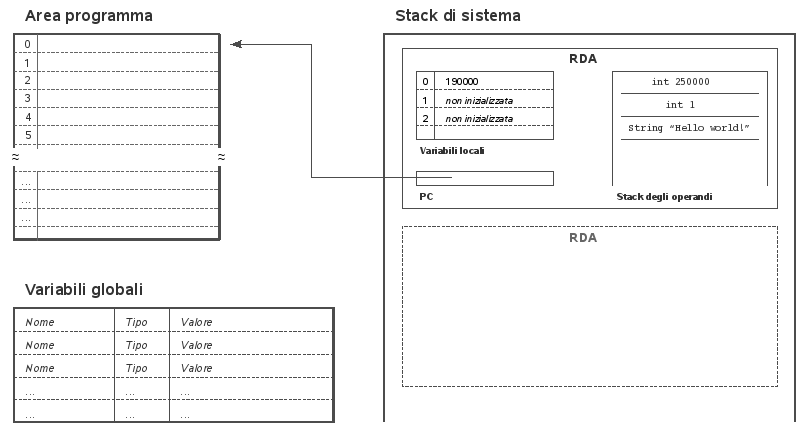
\includegraphics[width=\columnwidth]{graphics/struttura_generale.png}
\end{center}
Nell'\textbf{area programma} ci sono le istruzioni del programma divise in funzioni ed ogni istruzione ha un indice univoco e consecutivo all'istruzione che la precede. Nello spazio \textbf{variabili globali} ci sono tutte le variabili globali con il loro valore, distinte in base al nome e al tipo. Lo \textbf{stack di sistema} contiene i RDA (record di attivazione): ogni funzione ha un suo RDA, una chiamata a funzione comporta l'inserimento di un nuovo RDA sullo \textbf{stack di sistema} e le istruzioni ``return'' tolgono un RDA dallo stack. Ogni RDA ha uno \textbf{stack degli operandi}, uno spazio per le \textbf{variabili locali} e un \textbf{PC} (program counter); lo \textbf{stack degli operandi} viene utilizzato dalle varie istruzioni (vedere il funzionamento delle istruzioni in \ref{sec:dettagli_istruzioni}); lo spazio delle \textbf{variabili locali} contiene fino a 65536 ``registri'' nei quali si possono memorizzare o leggere valori, rispettivamente con le istruzioni ``store'' e ``load''; infine il \textbf{PC} contiene l'indice dell'istruzione da eseguire dell'\textbf{area programma}.

\subsection{Funzionamento}
Vengono eseguiti una serie di passi iniziali per costruire e inizializzare le strutture dati della macchina astratta, dopodich\'e l'esecuzione passa ad una funzione ``esecutore'' che si occupa di eseguire le istruzioni del programma.

\subsubsection*{Inizio}
\begin{enumerate}
  \item Legge il file contenente il programma e carica le istruzioni (divise per funzioni) nella struttura dati \textbf{area programma}.
  \item Ricerca le variabili globali nel programma e le mette nello spazio \textbf{variabili globali}.
  \item Se esiste la funzione \texttt{<clinit>} (funzione per inizializzare le variabili globali) crea un RDA vuoto nello \textbf{stack di sistema}, imposta il PC alla prima istruzione della funzione \texttt{<clinit>}, passa il controllo alla funzione esecutore e, quando ha terminato, prosegue con il punto seguente. Se tale funzione non esiste prosegue con il punto seguente.
  \item Costruisce il primo RDA nello \textbf{stack di sistema} con lo stack degli operandi vuoto, le variabili locali non inizializzate e il PC che punta alla prima istruzione della funzione \texttt{main}.
  \item Passa il controllo all'\textbf{esecutore} che esegue le istruzioni puntate dal PC e termina quando lo \textbf{stack di sistema} \`e vuoto (l'istruzione \texttt{return} toglie un RDA dallo stack).
\end{enumerate}

\subsubsection*{Esecutore}
\begin{enumerate}
  \item Controlla se lo \textbf{stack di sistema} \`e vuoto. Se non \`e vuoto continua, altrimenti termina l'esecuzione.
  \item Prende il valore del PC del RDA in cima allo \textbf{stack di sistema}.
  \item Legge l'istruzione puntata dal PC.
  \item Incrementa il PC.
  \item Esegue l'istruzione seguendo le specifiche in \ref{sec:dettagli_istruzioni}.
  \item Ritorna al punto 1.
\end{enumerate}
